\section{Arista}

\subsection{Introduction}

Arista Networks is an industry leader and present in many financial organizations, enterprises, and Fortune 500 companies. It is heavily used by carriers and organizations with demanding networks. 

While there is no Arista equipment in Rubin's network, some of the partners of the LHN have many Arista deployments and posees extensive experience on it. 

The quotations have been made by an Arista partner, and can be found in the following link <insert link>

\subsection{Hardware}

The hardware offered by the vendor is the \href{https://www.arista.com/assets/data/pdf/Datasheets/7260X3_Datasheet.pdf}{7260X3-64}, some of its features are:
\begin{itemize}
    \item 64 x QSFP100 (support for 10G or 100G)
    \item 2RU
    \item Up to 12.8 terabits per second
    \item Latency from 450ns
    
\end{itemize}

\begin{figure}
    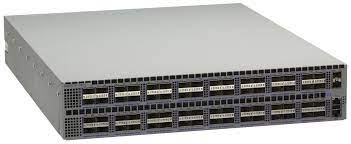
\includegraphics[width=11cm]{images/arista_7260X3-64.jpg}
    \centering
    \caption{Arista 7260X3-64}
  \end{figure}

\subsection{License}
\subsection{Network Design}
\subsection{Support}
\subsection{Training}
\subsection{Pros}
\subsection{Cons}
\subsection{Closing Comments}